% fig_study_system.tex — fragment (\input-able, no standalone wrapper)
\definecolor{busColor} {RGB}{ 30,  30,  30}
\definecolor{genColor} {RGB}{ 31, 119, 180}
\definecolor{ibrColor} {RGB}{ 44, 160,  44}
\definecolor{lineColor}{RGB}{ 80,  80,  80}
\definecolor{ctColor}  {RGB}{180,  30,  30}
\definecolor{zColor}   {RGB}{100,  60, 160}
\definecolor{relColor} {RGB}{180,  30,  30}
\tikzset{
  bus/.style      = {line width=3pt, color=busColor, line cap=round},
  zbox/.style     = {rectangle, rounded corners=2pt,
                     draw=#1, fill=#1!12, text=#1,
                     line width=0.8pt, font=\small, inner sep=4pt, align=center},
  ctcirc/.style   = {circle, draw=ctColor, fill=ctColor!15,
                     line width=0.9pt, inner sep=0pt, minimum size=14pt,
                     font=\tiny\bfseries, text=ctColor},
  lbl/.style      = {font=\scriptsize, align=center, color=gray!55!black},
  mainline/.style = {line width=1.2pt, color=lineColor},
  brace/.style    = {decorate,
                     decoration={brace, amplitude=5pt, raise=3pt},
                     line width=0.8pt},
}
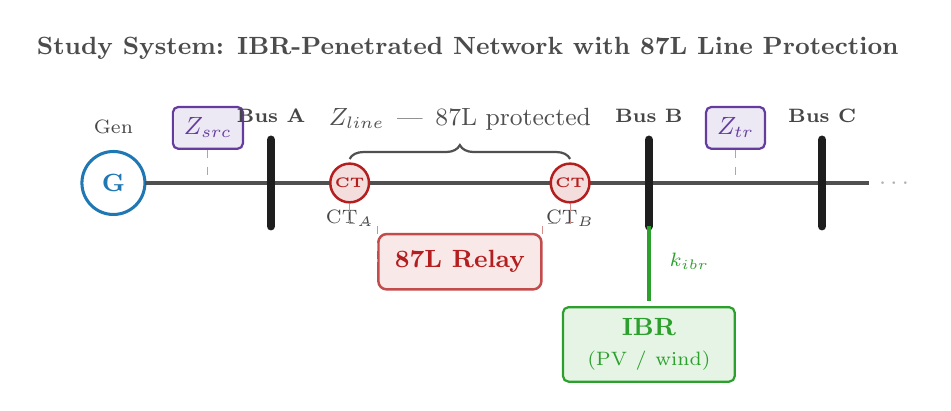
\begin{tikzpicture}

\def\yM{0}
\def\busH{0.55}

% x positions
\def\xGen{0}
\def\xBusA{2.0}
\def\xCTA{3.0}
\def\xCTB{5.8}
\def\xBusB{6.8}
\def\xBusC{9.0}

% ---- Generator --------------------------------------------------------------
\draw[genColor, line width=1.1pt] (\xGen,\yM) circle (0.40cm);
\node[font=\small\bfseries, text=genColor] at (\xGen,\yM) {G};
\node[lbl, above=0.50cm] at (\xGen,\yM) {Gen};

% ---- Main horizontal conductor ----------------------------------------------
\draw[mainline] ({\xGen+0.40},\yM) -- (\xBusA,\yM);
\draw[mainline] (\xBusA,\yM) -- ({\xCTA-0.07},\yM);
\draw[mainline] ({\xCTA+0.07},\yM) -- ({\xCTB-0.07},\yM);
\draw[mainline] ({\xCTB+0.07},\yM) -- (\xBusB,\yM);
\draw[mainline] (\xBusB,\yM) -- (\xBusC,\yM);
\draw[mainline] (\xBusC,\yM) -- ({\xBusC+0.6},\yM);
\node[font=\small, text=gray!60, anchor=west] at ({\xBusC+0.6},\yM) {\ldots};

% ---- Z_src (above line between Gen and Bus_A) --------------------------------
\node[zbox=zColor] (zsrc) at ({(\xGen+0.40+\xBusA)/2}, {\yM+0.70}) {$Z_{src}$};
\draw[zColor!50, thin, dashed] (zsrc.south) -- ({(\xGen+0.40+\xBusA)/2},\yM);

% ---- Bus_A ------------------------------------------------------------------
\draw[bus] (\xBusA,{\yM-\busH}) -- (\xBusA,{\yM+\busH});
\node[lbl, above=0.65cm] at (\xBusA,\yM) {\textbf{Bus A}};

% ---- CT_A -------------------------------------------------------------------
\node[ctcirc] (cta) at (\xCTA,\yM) {CT};
\node[lbl, below=0.22cm] at (\xCTA,\yM) {CT$_A$};

% ---- CT_B -------------------------------------------------------------------
\node[ctcirc] (ctb) at (\xCTB,\yM) {CT};
\node[lbl, below=0.22cm] at (\xCTB,\yM) {CT$_B$};

% ---- Z_line label: brace above protected segment + label --------------------
\draw[brace, color=lineColor]
  (\xCTA,{\yM+0.20}) -- (\xCTB,{\yM+0.20});
\node[font=\small, text=lineColor, anchor=south]
  at ({(\xCTA+\xCTB)/2},{\yM+0.55})
  {$Z_{line}$\enspace\textemdash\enspace 87L protected};

% ---- Bus_B ------------------------------------------------------------------
\draw[bus] (\xBusB,{\yM-\busH}) -- (\xBusB,{\yM+\busH});
\node[lbl, above=0.65cm] at (\xBusB,\yM) {\textbf{Bus B}};

% ---- IBR branch (downward from Bus_B) ----------------------------------------
\draw[mainline, draw=ibrColor] (\xBusB,{\yM-\busH}) -- (\xBusB,{-1.5});
\node[zbox=ibrColor, text width=1.9cm] at (\xBusB,{-2.05})
  {\textbf{IBR}\\{\scriptsize(PV / wind)}};
\node[lbl, right=4pt] at (\xBusB,{-1.0}) {\color{ibrColor}$k_{ibr}$};

% ---- Z_tr (above line between Bus_B and Bus_C) --------------------------------
\node[zbox=zColor] (ztr) at ({(\xBusB+\xBusC)/2},{\yM+0.70}) {$Z_{tr}$};
\draw[zColor!50, thin, dashed] (ztr.south) -- ({(\xBusB+\xBusC)/2},\yM);

% ---- Bus_C ------------------------------------------------------------------
\draw[bus] (\xBusC,{\yM-\busH}) -- (\xBusC,{\yM+\busH});
\node[lbl, above=0.65cm] at (\xBusC,\yM) {\textbf{Bus C}};

% ---- 87L Relay box below protected line -------------------------------------
\node[rectangle, rounded corners=3pt,
      draw=relColor!80, fill=relColor!10, text=relColor,
      line width=0.9pt, font=\small\bfseries, inner sep=6pt]
  (relay) at ({(\xCTA+\xCTB)/2},{-1.0}) {87L Relay};
% Dashed links from CTs to relay
\draw[relColor!50, thin, dashed]
  (cta.south) -- ++(0,-0.25) -| (relay.west);
\draw[relColor!50, thin, dashed]
  (ctb.south) -- ++(0,-0.25) -| (relay.east);

% ---- Title ------------------------------------------------------------------
\node[font=\small\bfseries, text=black!70, anchor=south]
  at ({(\xGen+\xBusC)/2},{1.45})
  {Study System: IBR-Penetrated Network with 87L Line Protection};

\end{tikzpicture}
